\documentclass[../main/main.tex]{subfiles}

\raggedbottom

\makeatletter
\renewcommand{\@chapapp}{Optique -- chapitre}
\makeatother

\begin{document}
\setcounter{chapter}{3}

\chapter{Dispositifs optiques}

\section{Œil}
\subsection{Présentation et modélisation}
Un œil est constitué de trois parties~:\smallbreak
\begin{tcbraster}[raster columns=2, raster equal height=rows]
    \begin{nota}[label=nota:oeilvoca]{Vocabulaire}
        \begin{description}
            \item[L'iris,] partie colorée, est percé de la pupille dont le diamètre est
                variable (\SIrange{2}{8}{mm}). Il joue le rôle de \textit{diaphragme},
                permettant de limiter la puissance lumineuse pénétrant dans
                l'œil\footnote{On pourra penser à Stargate SG1 avec la porte des étoiles
                protégée par un iris.}~;
            \item[Le cristallin,] milieu transparent ayant un effet de lentille mince,
                accroché à des muscles permettant d'en changer la focale selon leur
                contraction~;
            \item[La rétine,] l'«~écran~» de l'œil, constituée de cellules sensibles à
                la lumière (les cônes et les bâtonnets).
        \end{description}
        \begin{center}
            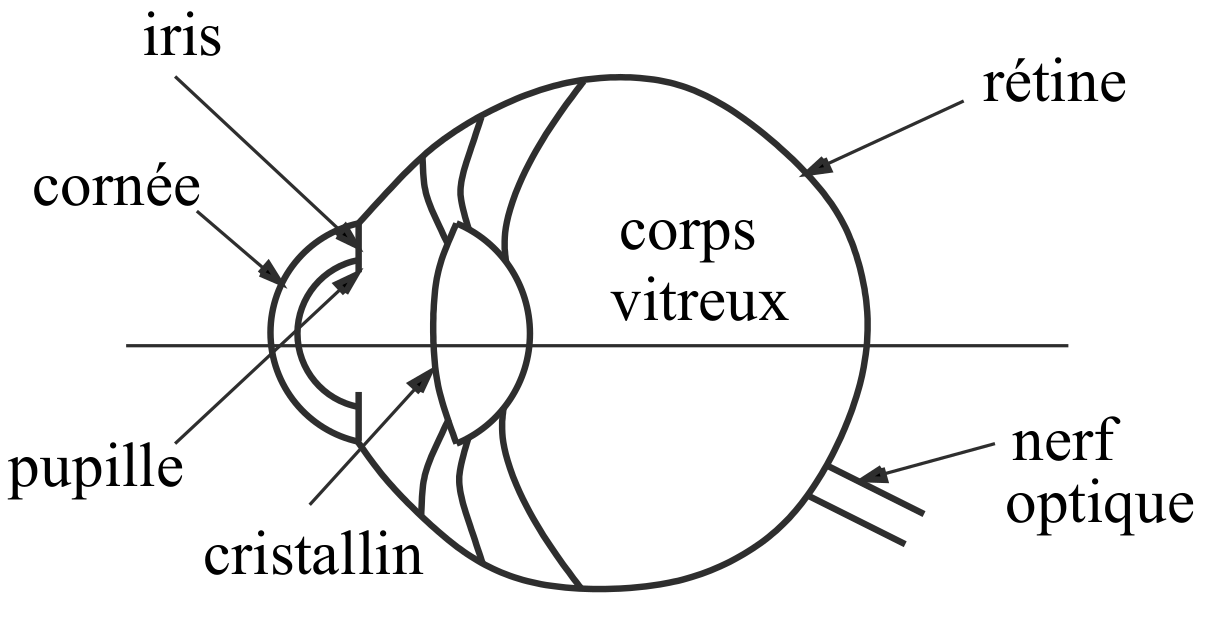
\includegraphics[width=\linewidth]{oeil_coupe}
            \captionof{figure}{Structure de l'œil.}
            \label{fig:oeil_coupe}
        \end{center}
    \end{nota}
    \begin{defi}[label=def:oeil]{modèle de l'œil}

        En optique, on le décrit donc par une \textbf{lentille mince convergente} de
        \textbf{vergence variable} associée à un \textbf{écran fixe}, telle que $d
        \approx \SI{22.3}{mm}$.
        \tcblower
        \begin{center}
            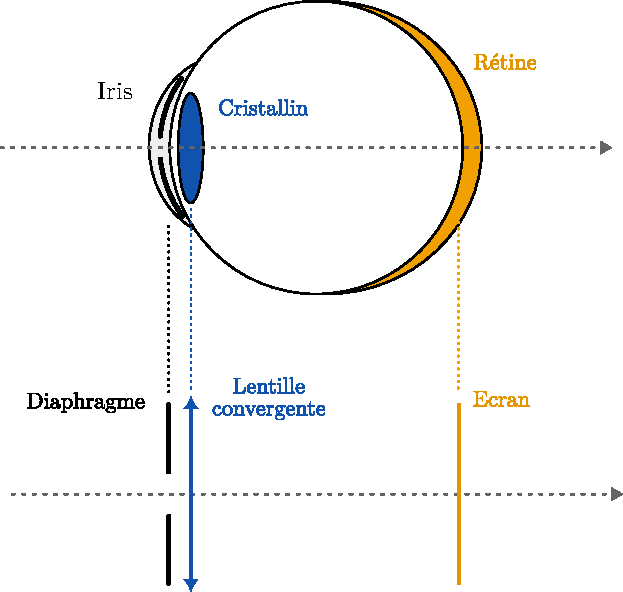
\includegraphics[width=\linewidth]{oeil_modele}
            \captionof{figure}{Modèle de l'œil en optique.}
            \label{fig:oeil_modele}
        \end{center}
    \end{defi}
\end{tcbraster}

\subsection{Caractéristiques}

\subsubsection{Plage d'accommodation}
L'œil ne voit net que si l'image se forme sur la rétine, comme pour tout
dispositif optique avec un écran. Selon la distance de l'objet à une
lentille, on a vu dans le chapitre 3 que la distance de l'image pouvait varier~:
ainsi, pour toujours voir net, un œil fait varier la vergence du cristallin pour
s'accommoder, en augmentant sa vergence (lentille $\oplus$ convergente) pour les
objets proches.
\begin{tcbraster}[raster columns=2, raster equal height=rows]
    \begin{defi}[label=def:pppr]{{punctum remotum, proximum}}

        %\begin{defiside}
            On appelle \textbf{punctum remotum} (PR) le point objet \textbf{le plus
            éloigné} qu'un œil voit \textit{net}.
            %\tcblower
            \tcbsubtitle[before skip=\baselineskip, colback=green!50!black,
            colframe=green!50!black]{Valeur}

            Pour un œil \textbf{sans défaut} (emmétrope), le PR est \textbf{à
            l'infini}.
        %\end{defiside}

        \tcblower
        %\begin{defiside}
            On appelle \textbf{punctum proximum} (PP) le point objet \textbf{le plus
            proche} qu'un œil voit \textit{net}.

            %\tcblower
            \tcbsubtitle[before skip=\baselineskip, colback=green!50!black,
            colframe=green!50!black]{Valeur}

            Pour un œil \textbf{sans défaut} (emmétrope), le PP est à $\approx$
            \textbf{\SI{25}{cm}}.

        %\end{defiside}
    \end{defi}
    \begin{NCexem}[width=\linewidth]{Schéma exemple}
        \begin{center}
            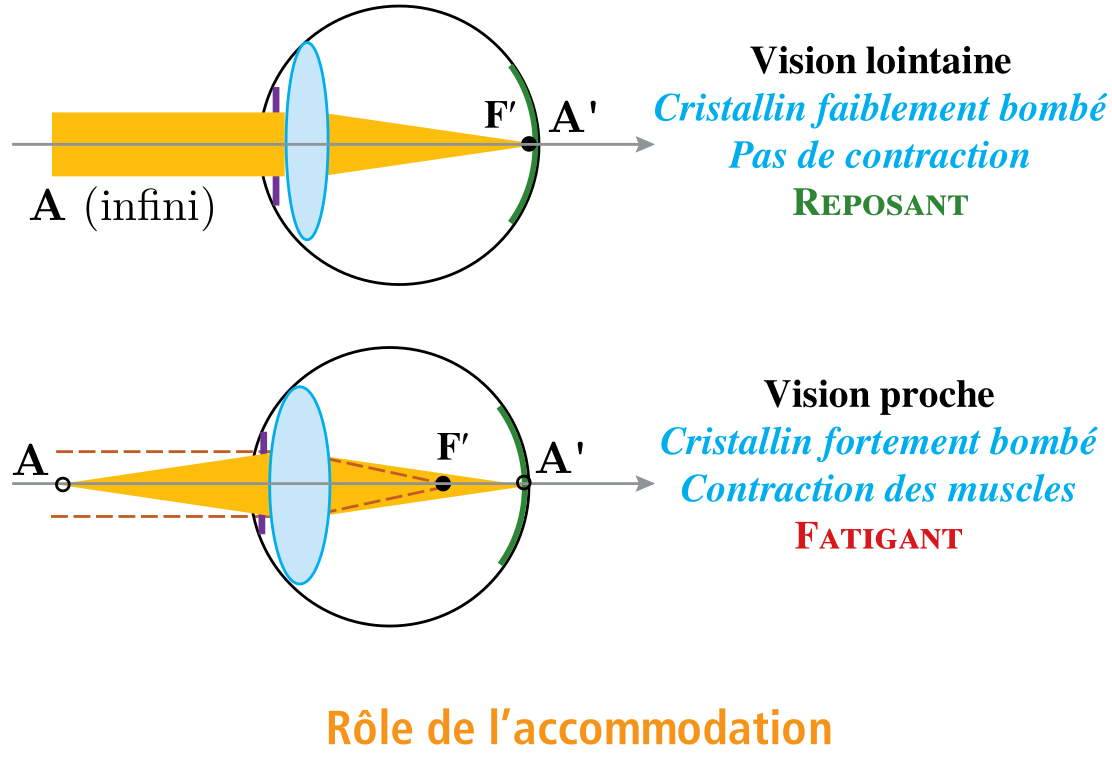
\includegraphics[width=\linewidth]{oeil_acco}
            \label{fig:oeil_acco}
            \captionof{figure}{Principe de l'accommodation d'un œil.}
        \end{center}
    \end{NCexem}
\end{tcbraster}

\begin{NCexem}[width=\linewidth]{Exercice~:}
    Quelles sont les valeurs maximale et minimale de la focale du cristallin
    pour un œil emmétrope~? On rappelle que la distance cristallin-rétine est $d
    \approx \SI{22.3}{mm}$.
    \tcblower
    \vspace{4cm}
\end{NCexem}

\begin{impl}[label=impl:instrument_opt]{réglage instrument optique}
    Le principe des instruments optiques est d'avoir de meilleures
    caractéristiques que l'œil humain, mais que l'image formée soit visible par
    un œil. Pour que cela se fasse sans fatigue,
    \begin{center}
        \bfseries L'image finale d'un instrument d'optique doit être à l'infini.
    \end{center}
\end{impl}

\subsubsection{Résolution angulaire}
Comme tout capteur, l'œil distingue deux points sources si leurs images se
forment sur deux cellules différentes de la rétine. On caractérise cette
capacité par le pouvoir de résolution.
\begin{tcbraster}[raster columns=2, raster equal height=rows]
    \begin{defi}[label=def:resolu]{pouvoir de résolution}
        Le pouvoir de résolution (ou séparateur) d'un capteur optique est l'angle
        minimal que doivent former deux rayons pour être perçus comme provenant de
        deux points différents.
    \end{defi}
    \begin{odgr}[label=odgr:resolu]{résolution}

        Dans de bonnes conditions d'éclairement (luminosité moyenne), le pouvoir
        séparateur d'un œil emmétrope est \fbox{$\alpha \approx\ang{;1;} =
        \SI{3e-4}{rad}$}. Cela revient à distinguer deux détails séparés de
        \SI{1}{mm} à une distance de \SI{3}{m}.
    \end{odgr}
\end{tcbraster}

\subsubsection{Défauts de l'œil}
\begin{tcbraster}[raster columns=2, raster equal height=rows]
    \begin{defi}[label=def:defaut_oeil]{défauts de l'œil}
        \begin{description}
            \item[Myopie] : cristallin \textbf{trop} convergent. PR pas à
                l'infini. Corrigé par lentille divergente.
            \item[Hypermétropie] : cristallin \textbf{pas assez} convergent. PP
                plus éloigné que l'œil emmétrope. Corrigé avec lentille
                convergente.
            \item[Presbytie] : les muscles du cristallin vieillissent et ont du
                mal à accommoder. Pour la faciliter, on utilise une lentille
                convergente.
        \end{description}
    \end{defi}
    \begin{NCexem}[width=\linewidth]{Schéma}
        \begin{center}
            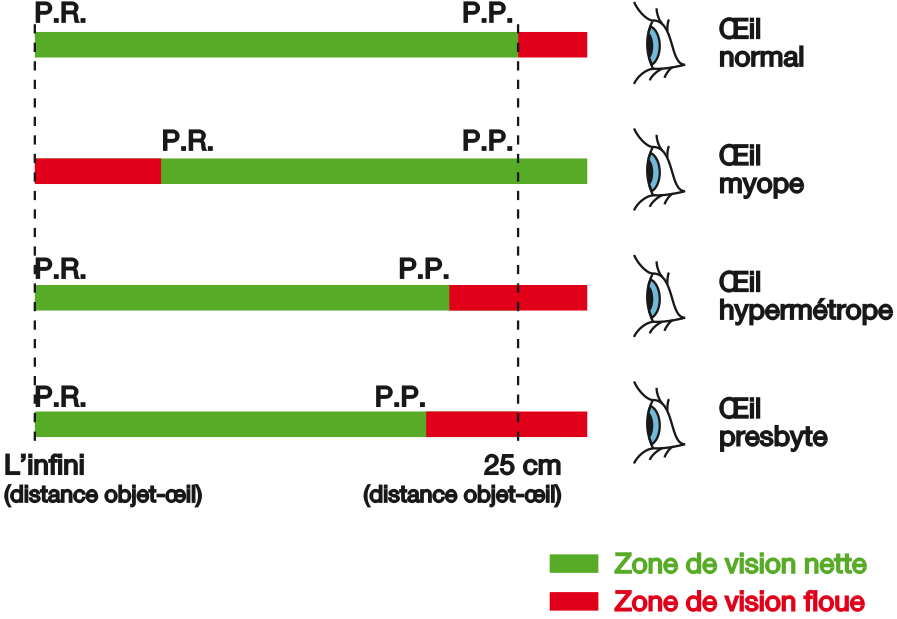
\includegraphics[width=\linewidth]{oeil_defaut}
            \captionof{figure}{Schéma des défauts de l'œil.}
            \label{fig:oeil_defaut}
        \end{center}
    \end{NCexem}
\end{tcbraster}

\section{La loupe}
Le point le plus proche permettant une vision nette étant fixé (PP), pour mieux
voir un objet, il faut utiliser un instrument~: c'est ce que permet la loupe.

\begin{defi}[label=def:loupe, valign=center]{effet loupe et accommodation}
    \begin{tcolorbox}[sidebyside, sidebyside align=center,
    enhanced, colback=green!10!, colframe=green!60!black, valign=center,
    arc=0pt, boxsep=1mm, notitle, oversize, nobeforeafter, frame hidden,
    righthand width=.5\linewidth]
        Pour obtenir l'effet loupe, il faut que l'objet soit situé entre le
        \textbf{centre optique} d'une lentille \textit{convergente} et son
        \textbf{foyer objet}~: on obtient alors une image \textbf{virtuelle},
        \textbf{droite} et \textbf{agrandie}.
        \vfill
        \tcblower
        \begin{center}
            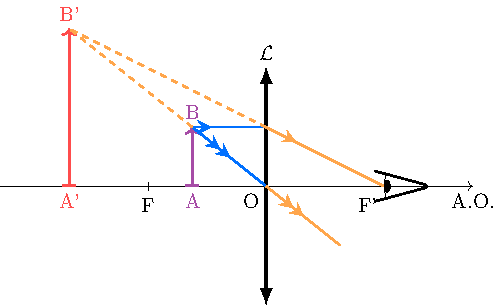
\includegraphics[width=\linewidth]{loupe}
            \captionof{figure}{Loupe avec accommodation}
            \label{loupeavecacc}
        \end{center}
    \end{tcolorbox}
    \tcblower
    \begin{tcolorbox}[sidebyside, sidebyside align=center,
    enhanced, colback=green!10!, colframe=green!60!black, valign=center,
    arc=0pt, boxsep=1mm, notitle, oversize, nobeforeafter, frame hidden,
    righthand width=.5\linewidth]
        
        De plus, afin que l'œil puisse observer cette image sans accommodation,
        celle-ci doit être \textbf{à l'infini}. La meilleure position de l'objet
        est celle où il sera \textbf{sur le foyer principal objet}.

        \tcblower
        \begin{center}
            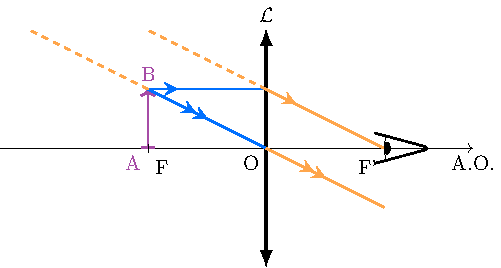
\includegraphics[width=\linewidth]{loupeparfaite}
            \captionof{figure}{Loupe sans accommodation}
            \label{loupesansacc}
        \end{center}

    \end{tcolorbox}
\end{defi}

\paragraph*{L'image obtenue avec une loupe peut-elle être plus ou moins grande~?
La distance objet-lentille joue-t-elle sur la taille de l'image
observée~?\newline\newline}

\begin{minipage}[c]{0.45\linewidth}
    La réponse est non~:
    \begin{itemize}
        \item Si on approche l'objet de la lentille, l'image devient moins
            grande (voir figure \ref{loupeplusieursobjets}), mais elle est vue
            plus près ;
        \item Si on éloigne l'objet de la lentille (en gardant $|\obar{OA}| <
            |\obar{OF}|$ , l'image devient plus grande (voir figure
            \ref{loupeplusieursobjets}), mais elle est vue plus loin !
    \end{itemize}
    \medskip
    L'angle $\theta'$ défini sur cette figure est le même quel que soit le cas,
    il ne dépend que de la lentille~: avec les dispositifs optiques, c'est cet
    angle qui est notre grandeur d'intérêt, plutôt que le grandissement
    transversal qui vaut pour une image sur un écran.

\bigskip

\end{minipage}
\hfill 
\begin{minipage}[c]{0.45\linewidth}
    \begin{center}
        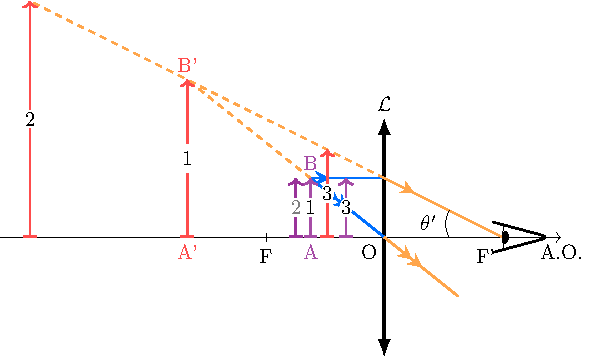
\includegraphics[width=\linewidth]{loupe_objets}
        \captionof{figure}{Image obtenue avec une loupe dans plusieurs cas de
        distance objet-lentille}
        \label{loupeplusieursobjets}
    \end{center}
\end{minipage}

\bigskip

\begin{tcbraster}[raster columns=3, raster equal height=rows]
    \begin{defi}[label=def_gross, raster multicolumn=2, sidebyside]{grossissement}

        On définit alors le grossissement d'un dispositif optique par le rapport 
        \begin{equation*}
            \boxed{G = \frac{\theta'}{\theta}}
        \end{equation*}
        Avec
        \begin{itemize}
            \item L'angle $\theta'$ sous lequel est vu l'image~;
            \item L'angle $\theta$ sous lequel est vu l'objet depuis l'œil à la
                distance de vision minimale de l'œil emmétrope soit $d_m
                = \SI{25}{cm}$.
        \end{itemize}
        \tcblower
        \begin{center}
            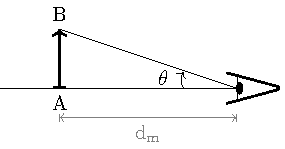
\includegraphics[width=\linewidth]{thetaobj}
            \captionof{figure}{Définition de $\theta$}
            \label{thetaobj}
        \end{center}
        \begin{center}
            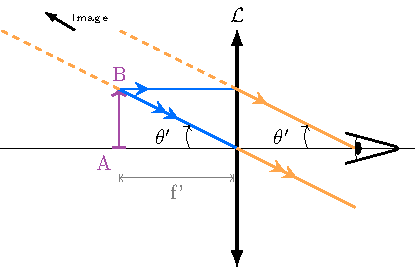
\includegraphics[width=\linewidth]{thetaimg}
            \captionof{figure}{Définition de $\theta'$}
            \label{thetaimg}
        \end{center}
    \end{defi}
    \begin{tcolorbox}[blankest, raster multicolumn=1]
        \begin{tcbraster}[raster columns=1]
            \begin{prop}[label=prop_loupe]{loupe et grossissement}
                Une loupe a un grossissement fixé, tel que
                \begin{equation*}
                    \boxed{G = \frac{d_m}{f'}}
                \end{equation*}
            \end{prop}
            \begin{demo}[label=demo_gross-loupe]{grossissement loupe}
                Avec les schémas~\ref{thetaobj} et \ref{thetaimg}, en
                appelant $h$ la hauteur de l'objet et en supposant qu'on a des
                petits angles ($\tan(\theta)\approx\theta$), on a
                \begin{equation*}
                    G = \frac{\theta'}{\theta} = \frac{\dfrac{h}{f'}}{\dfrac{h}{d_m}}
                    = \frac{d_m}{f'}
                \end{equation*}
            \end{demo}
        \end{tcbraster}
    \end{tcolorbox}
\end{tcbraster}

\section{L'appareil photo réflex}

\subsection{Description}

\begin{defi}[label=def:reflex, %sidebyside,
    righthand width=.7\linewidth]{définition et schéma}
    
On appelle appareil photo réflex un appareil qui utilise un seul objectif pour
la visée et pour la prise de vue. Pour se faire, l'appareil utilise un miroir
plan incliné à \ang{45;;} sur l'axe optique de l'objectif et un pentaprisme~:

\begin{itemize}
    \item Pour la visée, le miroir plan renvoie la lumière vers le pentaprisme
        qui la transmet à l'œil par l'intermédiaire du viseur~;
    \item Lorsque la-e photographe appuie sur le déclencheur, ce miroir plan
        pivote de façon à laisser passer la lumière vers le capteur.
\end{itemize}
\tcblower
\begin{center}
	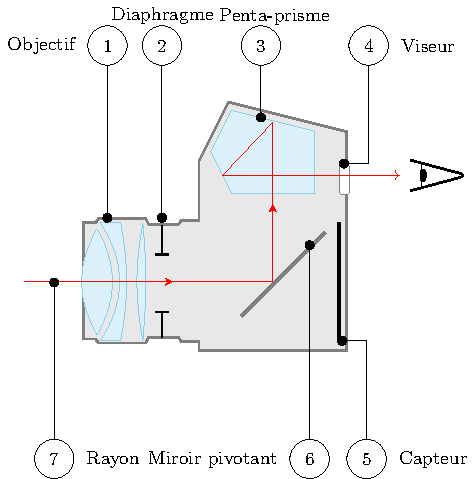
\includegraphics[width=\linewidth]{reflex}
    \captionof{figure}{Description d'un appareil photo réflex}
\end{center}
\end{defi}

\subsection{Champ d'un appareil photo}

Le champ d'un appareil photo est la portion d'espace qu'il peut photographier.
Celui-ci dépend de la focale de l'objectif, mais aussi de la taille du capteur.

\subsubsection{Influence de la focale de l'objectif}

Voici des photos prises du même endroit avec un appareil muni d'un unique
capteur mais avec des objectifs de focales différentes. À droite le schéma
illustrant chaque situation~:\newline

\begin{center}
    \begin{tabular}{cc} 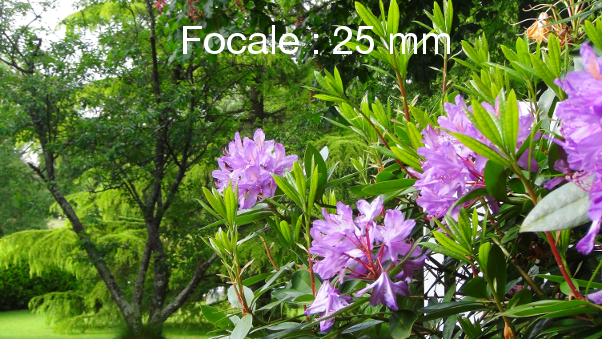
\includegraphics[height=4cm]{focale-25mm.png} & 
        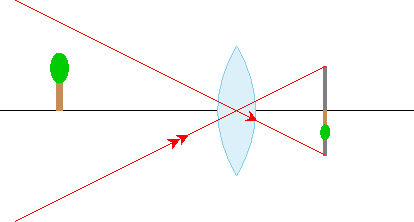
\includegraphics[width=.5\linewidth]{focale_obj-a} \\
        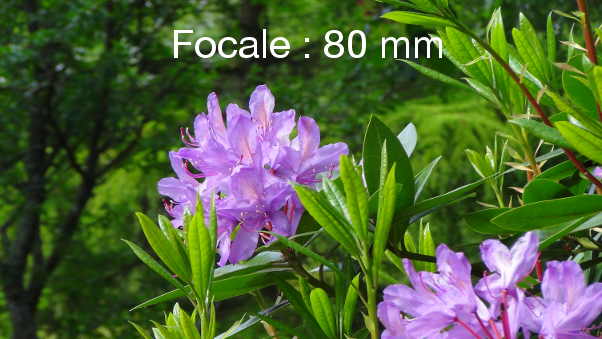
\includegraphics[height=4cm]{focale-80mm.png} & 
        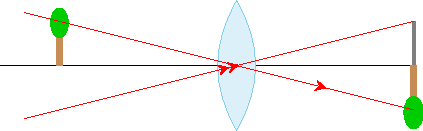
\includegraphics[width=.5\linewidth]{focale_obj-b} \\
    \end{tabular}
\end{center}

\medskip

\textbf{Donc plus la focale est grande, plus le champ est étroit, plus on
capture un détail de l'image.}\newline

On dit que la première photo est prise avec un grand angle (focale courte,
encombrement de l'appareil minimum), la deuxième est prise avec un téléobjectif
(focale longue, encombrement important).

\subsubsection{Influence de la taille du capteur}

Voyons maintenant ce qu'il se passe si on garde une focale de 25 mm (première
photo) mais que l'on diminue la taille du capteur. Sur des illustrations cela
donne~:

\begin{minipage}{0.49\linewidth}
    \begin{center}
         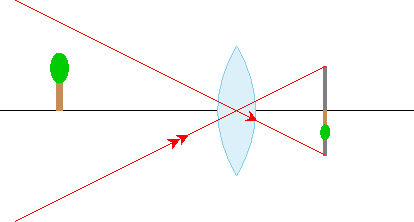
\includegraphics[scale=1]{taille_capt-a} \\
    \end{center}
\end{minipage}
\begin{minipage}{0.49\linewidth}
    \begin{center}
         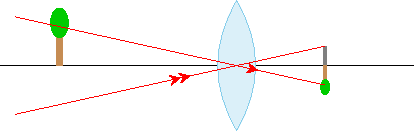
\includegraphics[scale=1]{taille_capt-b} \\
    \end{center}
\end{minipage}

\medskip

Ainsi, grand angle ne signifie pas forcément courte focale, car cela dépend de
la taille du capteur.\newline


\subsubsection{Focale réelle et équivalente}

Pour que tout le monde puisse identifier si un appareil sera un grand angle d'un
téléobjectif, on a inventé la focale équivalente. C'est une focale calculée pour
une seule taille de capteur (en l'occurrence un capteur $24 \times 36$). Si
cette focale équivalente est grande, on a un téléobjectif, si elle est petite,
on a un grand angle. C'est généralement cette focale équivalente qui est
annoncée sur les appareils compacts à objectifs fixes.

\medskip

Pour les objectifs des réflex qui sont généralement interchangeables, on indique
sur ceux-ci leur focale réelle. On ne connaîtra donc le champ couvert par
l'appareil que si on associe cette valeur réelle à la taille du capteur. Les
fabricants d'appareils donnent alors le facteur de conversion permettant de
passer de la focale réelle de objectif à la focale équivalente de l'ensemble
objectif-capteur.\newline

\medskip

Voici alors l'utilisation des appareils selon leur focale équivalente~: 

\begin{minipage}{0.49\linewidth}
    \begin{itemize}[leftmargin=150pt]
        \item [\textbf{\SIrange{00}{60}{mm}}] grand angle ; 
        \item [\textbf{\SIrange{60}{120}{mm}}] focale à portrait ; 
    \end{itemize}
\end{minipage}
\begin{minipage}{0.49\linewidth}
    \begin{itemize}[leftmargin=70pt]
        \item [\textbf{\SIrange{40}{60}{mm}}] standard ; 
        \item [\textbf{\SIrange{60}{300}{mm}}] téléobjectif.
    \end{itemize}
\end{minipage}

\subsection{La mise au point}

Voici trois photos prises dans les mêmes conditions (même appareil, même focale,
même endroit de prise de vue) mais avec trois mises au point différentes~:
\begin{center}
    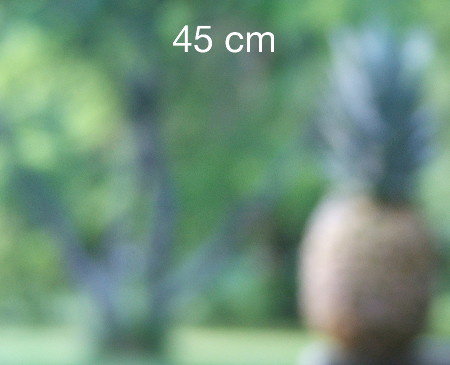
\includegraphics[height=3cm]{miseaupt-45cm.png}
    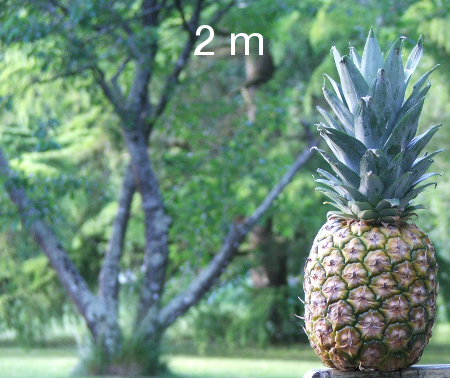
\includegraphics[height=3cm]{miseaupt-2m.png}
    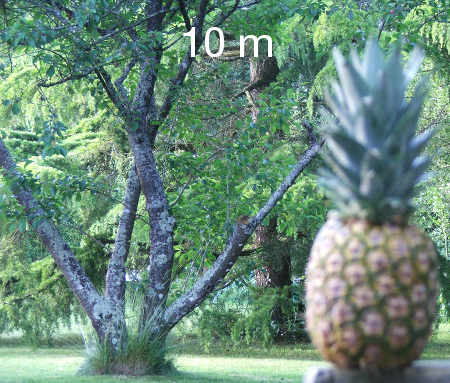
\includegraphics[height=3cm]{miseaupt-10m.png}
\end{center}

C'est elle qui détermine ce qui sera net sur la photo finale et ce qui ne le
sera pas. On la règle donc de façon à choisir le sujet à photographier. Elle
peut se régler automatiquement (souvent en appuyant à mi-course sur le
déclencheur), ou bien manuellement via une bague qui tourne autour de
l'objectif. Sur cette bague, la mise au point est gradué en mètres~: «~je veux
faire la mise au point à 5 m de l'appareil~». Un objectif indique généralement
les distances minimales et maximales de mise au point. 

Prenons l'exemple d'une scène avec un humain situé devant un arbre~:

\begin{minipage}{0.53\linewidth}
    \begin{center}
        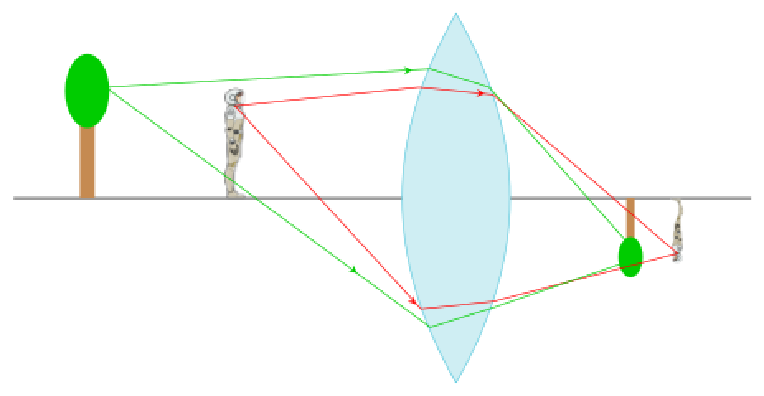
\includegraphics[width=\linewidth]{mise_pt-a}
    \end{center}    
\end{minipage}
\hfill
\begin{minipage}{0.45\linewidth}
    Je dois choisir qui je veux photographier. Si je choisis l'humain, je dois
    placer mon capteur au niveau de l'image de l'humain, les points objets de
    l'arbre donneront des taches images, ce qui donnera un arrière plan composé
    d'un arbre flou.
\end{minipage}

\begin{minipage}[c]{0.59\linewidth}
    \begin{center}
        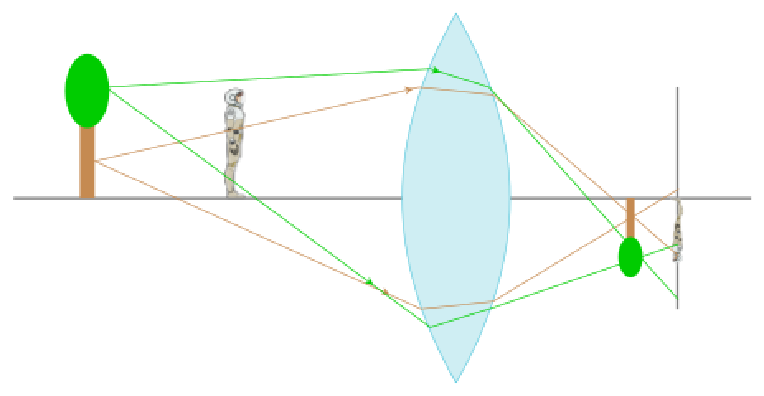
\includegraphics[scale=1]{mise_pt-b}
    \end{center}
\end{minipage}\hfill 
\begin{minipage}[c]{0.31\linewidth}
    \begin{center}
        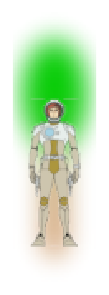
\includegraphics[scale=1]{mise_pt-res}
    \end{center}
\end{minipage}

Donc la bague de mise au point doit agir sur la position du capteur par rapport
à l'objectif pour sélectionner l'image à «~imprimer~» (dans le cas de l'humain,
je fais la mise au point sur un objet proche, je dois éloigner mon capteur de
l'objectif). Sur les appareils basiques, il y a vraiment déplacement, sur de
plus perfectionnés, des lentilles de l'objectif se déplacent pour obtenir la
mise au point voulue.

\subsection{La profondeur de champ}

\begin{center}
    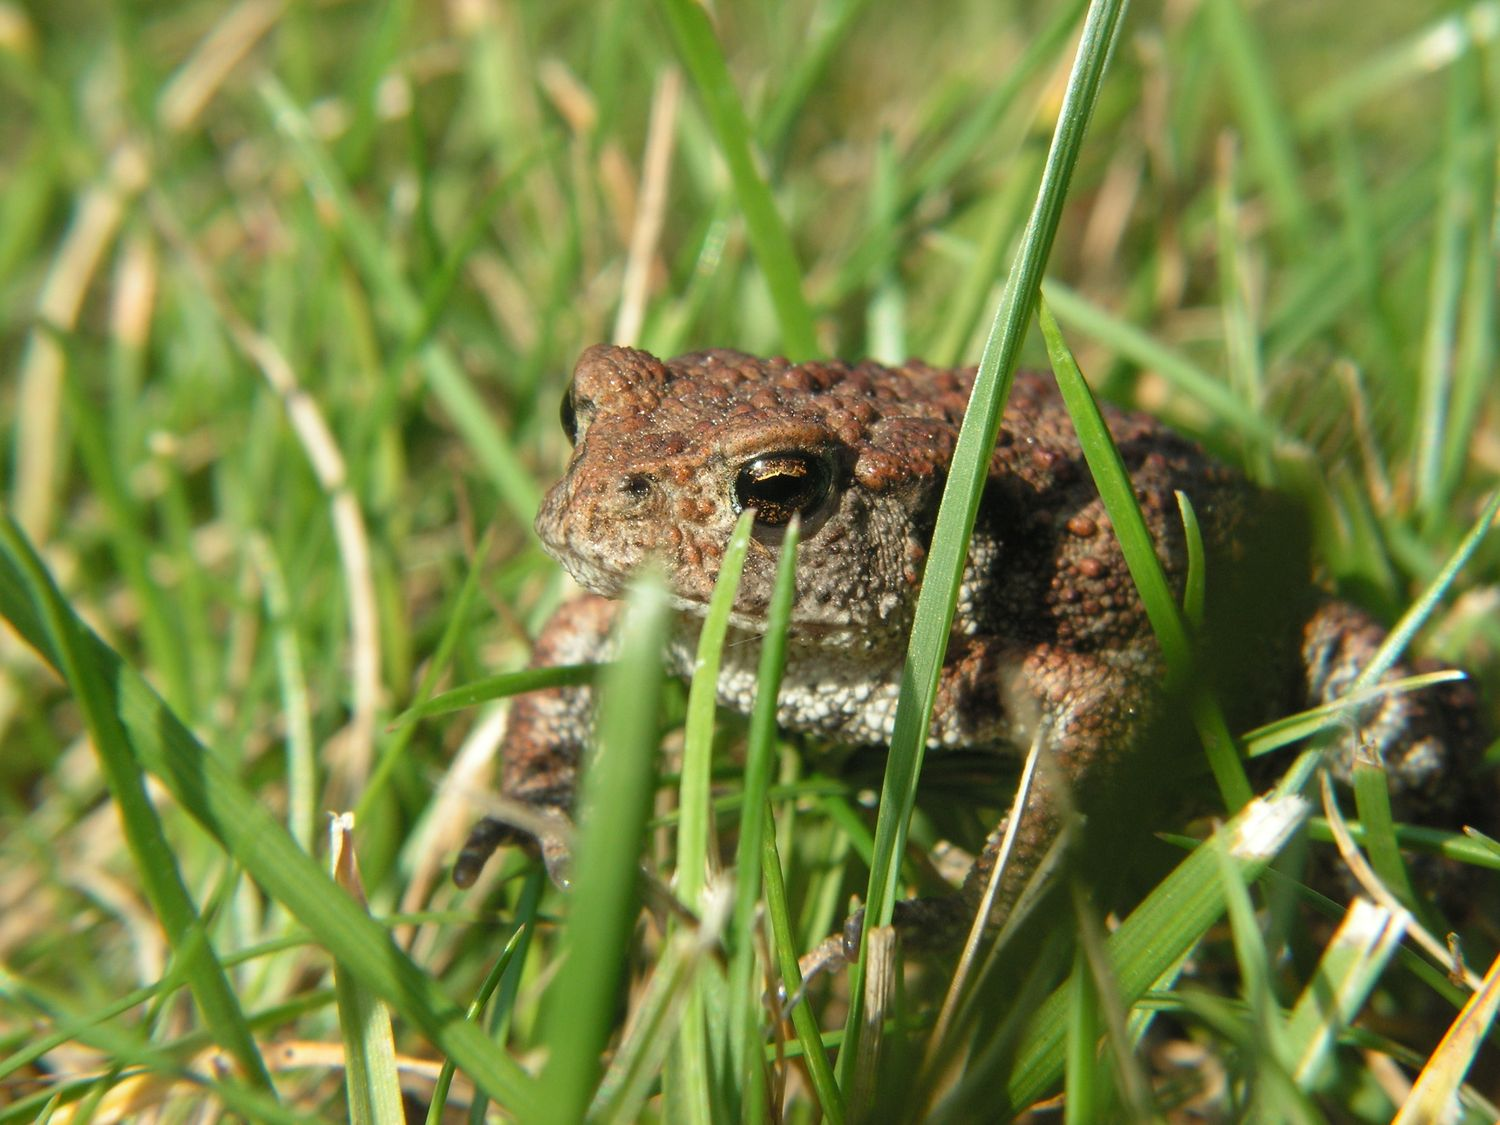
\includegraphics[scale=0.095]{photo-pdc-faible.jpg} \qquad
    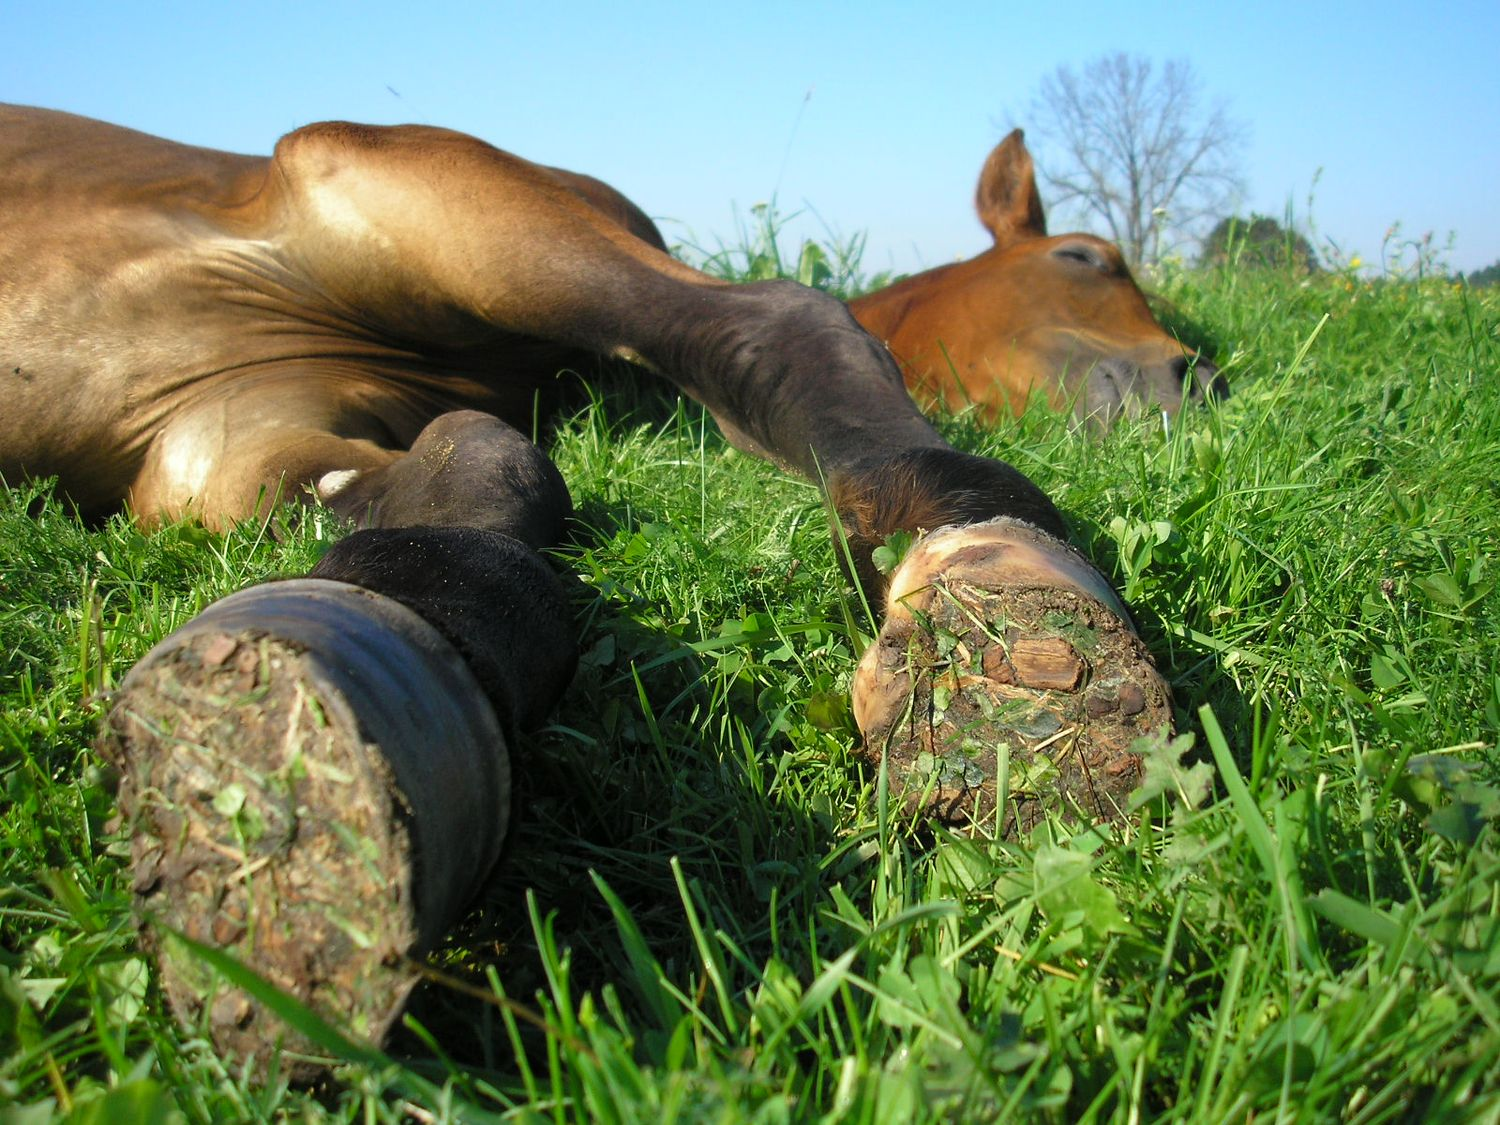
\includegraphics[scale=0.095]{photo-pdc-eleve.jpg}
\end{center}

Sur la première photo, nous voyons que le batracien est net, mais l'avant plan
et l'arrière plan sont flous, la profondeur de champ est faible. Sur la
deuxième, les sabots comme la tête de l'animal sont nets alors qu'ils ne sont
pas situés sur le même plan : la profondeur de champ est grande.

\begin{defi}[label=def:pdc]{profondeur de champ}
    
    La profondeur de champ est la distance entre les deux points objets extrêmes
    de l'axe optique dont les images sont vues nettes sur le capteur de
    l'appareil~; elle correspond à la zone de netteté en avant et en
    arrière du plan de mise au point~: plus celle-ci est grande, plus la
    profondeur de champ est grande. Elle dépend de l'ouverture, de la mise au
    point et de la focale.
\end{defi}

\subsubsection{Profondeur de champ et distance de mise au point} % (fold)
 
La profondeur de champ dépend de la distance de mise au point~: plus celle-ci est
grande, plus la profondeur de champ est grande comme le montre le schéma
suivant.

\begin{center}
	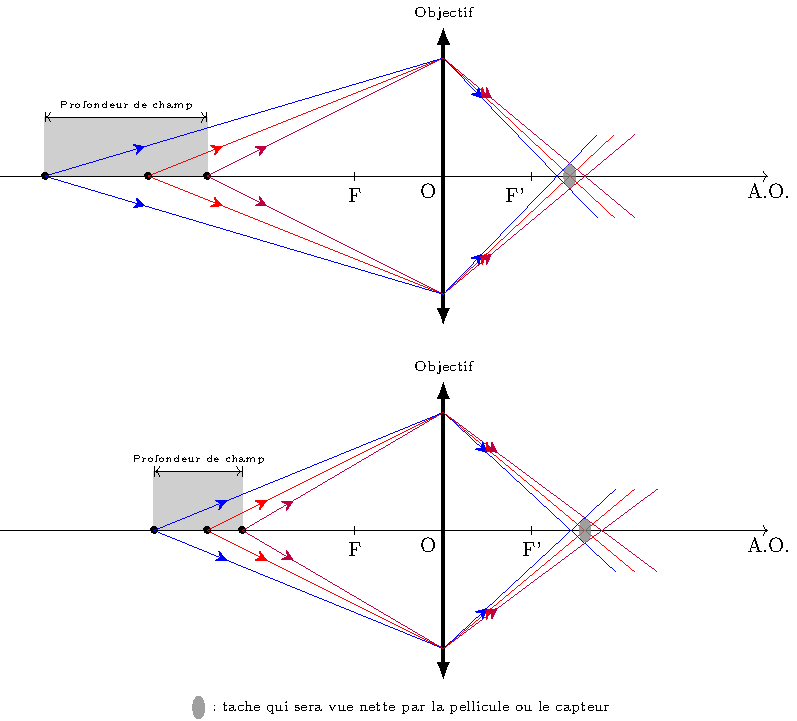
\includegraphics[scale=.95]{pfd_chp-map-a}
	\captionof{figure}{}
\end{center}

\subsubsection{Profondeur de champ et focale} % (fold)

De la même manière la profondeur de champ dépend de la focale~:

\begin{center}
	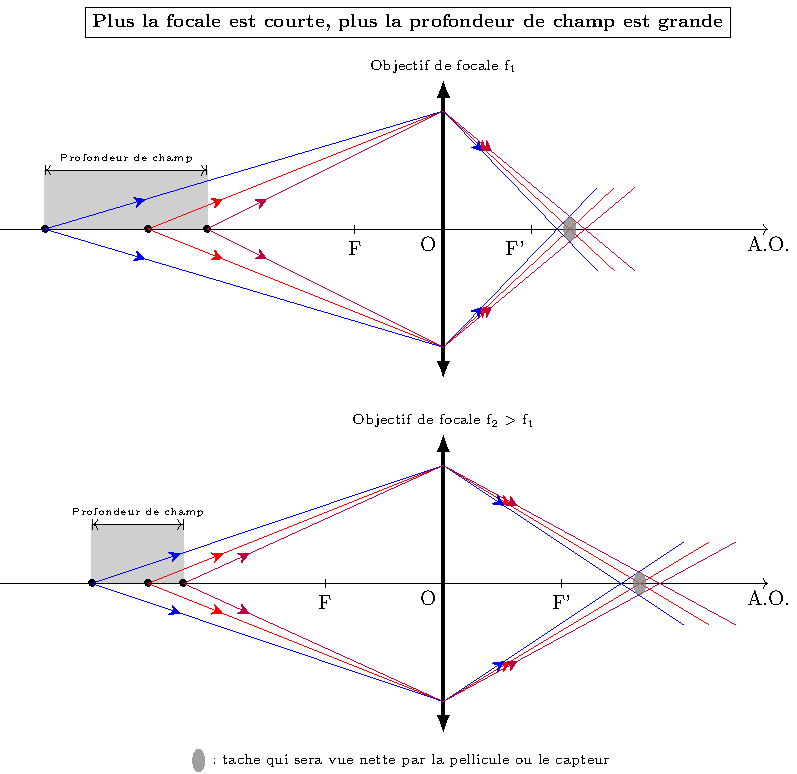
\includegraphics[scale=.95]{pfd_chp-foc}
	\captionof{figure}{}
\end{center}

\subsubsection{Profondeur de champ et ouverture} % (fold)

L'ouverture, c'est-à-dire le diamètre d'entrée de l'objectif, se règle à l'aide
d'un diaphragme. Plus l'ouverture est petite et plus la profondeur de champ sera
grande~; mais attention, la taille de l'ouverture influe sur la quantité de
lumière qui imprégnera le capteur. Cette ouverture est indiquée en fonction de
la focale de l'objectif~: une ouverture de $\frac{f}{22}$ est plus petite qu'une
ouverture de $\frac{f}{4}$.

Voici deux schémas qui montrent pourquoi la réduction de l'ouverture agrandit la
profondeur de champ~:

\begin{minipage}{0.47\linewidth}
    \begin{center}
        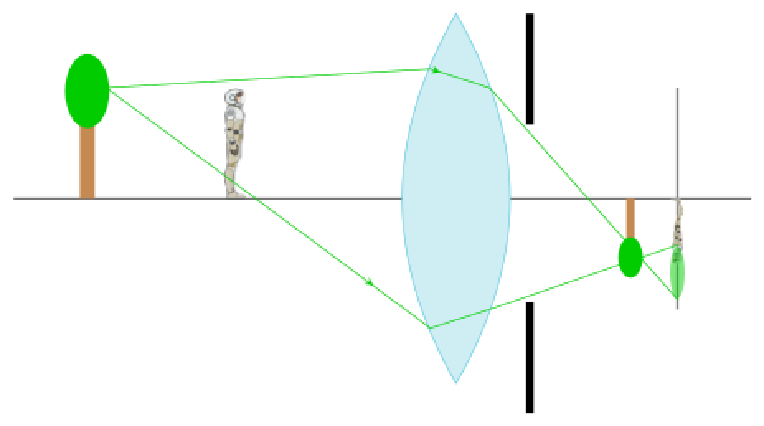
\includegraphics[width=\linewidth]{pfd_chp_ouverture-a}
        \captionof{figure}{}
    \end{center}
    Avec un diaphragme ouvert, les feuilles des arbres créent une tache
    lumineuse assez large sur le capteur, et ne seront pas vues nettes.
\end{minipage}
\hfill
\begin{minipage}{0.47\linewidth}
    \begin{center}
        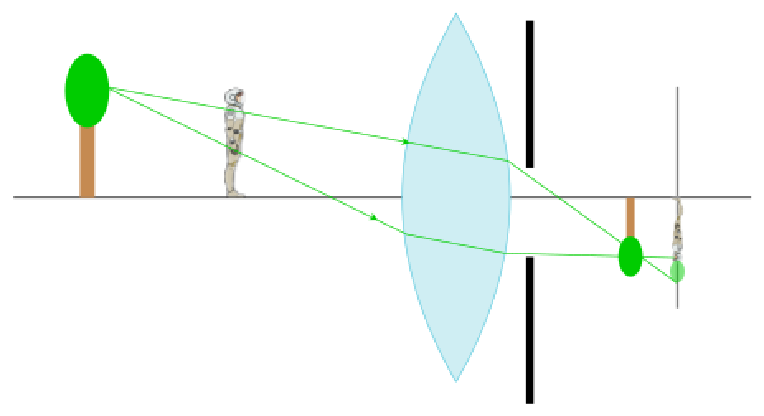
\includegraphics[width=\linewidth]{pfd_chp_ouverture-b}
        \captionof{figure}{}
    \end{center}
    En réduisant l'ouverture, cette tache est plus petite. Si elle est
    inférieure à la taille d'un pixel du capteur, les feuilles
    seront vues nettes.
\end{minipage}

\medskip

L'objet qui donnera une tache aussi grosse que les feuilles d'arbre du premier
schéma sera plus loin en avant ou en arrière de l'humain, la zone de netteté
sera plus réduite.

\subsubsection{Résumé et conclusion}
\begin{impo}[label=impo:app_phot]{résumé caractéristiques appareil photo}
    \begin{minipage}{0.50\linewidth}
        \begin{itemize}
            \item Focale $\nearrow\quad\Rightarrow$ champ $\searrow$~;
            \item Position capteur $\nearrow\quad\Rightarrow$ mise au point
                $\searrow$~;
            \item Taille capteur $\nearrow\quad\Rightarrow$ champ $\nearrow$~;
        \end{itemize}
    \end{minipage}
    \begin{minipage}{0.50\linewidth}
        \begin{itemize}
            \item Focale $\nearrow\quad\Rightarrow$ PDC $\searrow$~;
            \item Position capteur $\nearrow\quad\Rightarrow$ PDC $\searrow$~;
            \item Ouverture $\nearrow\quad\Rightarrow$ PDC $\searrow$.
        \end{itemize}
    \end{minipage}
\end{impo}

Typiquement, on utilise une profondeur de champ faible, donc une grande
ouverture pour effectuer des portraits, et une profondeur de champ importante
lorsqu'il s'agit de photographier un paysage.\newline
Mais en même temps que l'on règle celle-ci, il faut penser à régler le temps
d'exposition du capteur (le temps pendant lequel le miroir plan du reflex
pivotera), car la photo risquerait d'être sur-exposée (pour un portrait) ou
sous-exposée (pour un paysage).

\section{Systèmes optiques à plusieurs lentilles}

\subsection{Association quelconque de lentilles}
Les associations de lentilles ne présentent pas de difficultés particulières,
une fois les techniques de construction maîtrisées. Il faut cependant savoir
toujours se repérer dans les constructions.

\subsubsection{Entraînement}

\begin{exem}[label=exem:asso_lent]{association quelconque de lentilles
    convergentes}
    Deux lentilles minces convergentes $\Lc_1$ de centre optique $O_1$ et
    $\Lc_2$ de centre optique $O_2$ sont disposées selon le schéma ci-dessous.
    Trouver la position de l'image finale $A'B'$ de l'objet $AB$ donnée par
    l'association $\Lc_1 + \Lc_2$, et donner la nature de tous les objets et
    images.
    \tcblower
    \begin{center}
        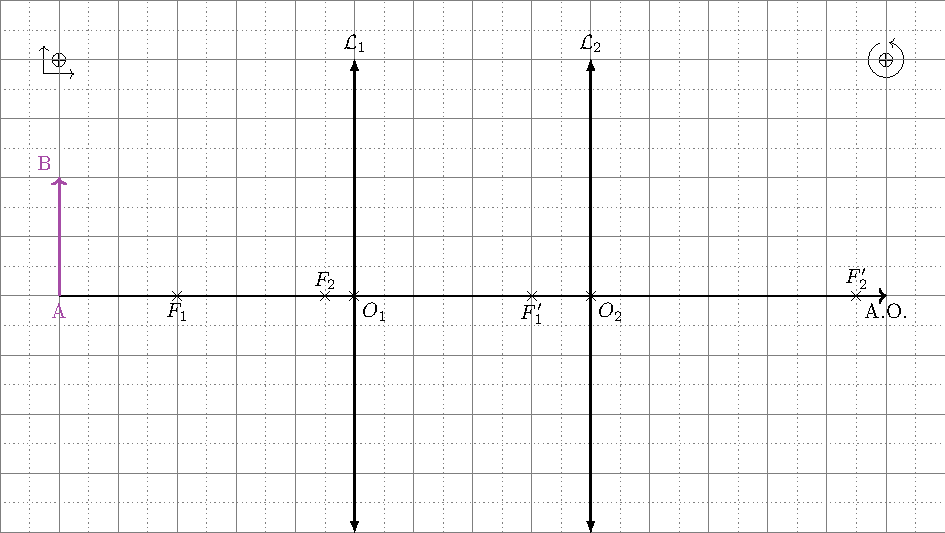
\includegraphics[width=.85\linewidth]{asso_lent-a_plain.pdf}
        \captionof{figure}{Association de lentilles convergentes}
        \label{fig:asso_lent-conv_plain}
    \end{center}
\end{exem}
\begin{exem}[label=exem:asso_lent]{association quelconque de lentilles
    mixées}

    Une lentille mince convergente $\Lc_1$ de centre optique $O_1$ et une
    divergente $\Lc_2$ de centre optique $O_2$ sont disposées selon le schéma
    ci-dessous. Trouver la position de l'image finale $A'B'$ de l'objet $AB$
    donnée par l'association $\Lc_1 + \Lc_2$, et donner la nature de tous les
    objets et images.

    \tcblower
    \begin{center}
        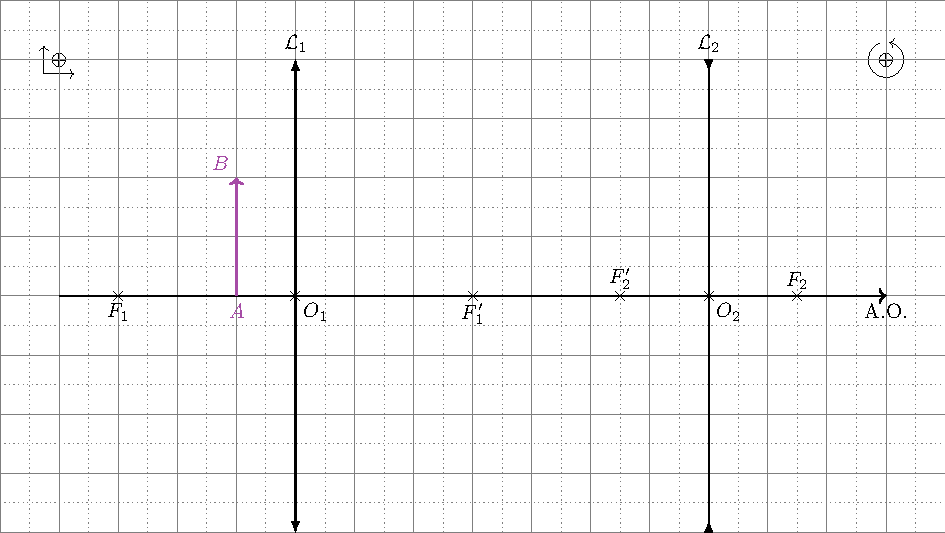
\includegraphics[width=.85\linewidth]{asso_lent-b_plain.pdf}
        \captionof{figure}{Association de lentilles mixées}
        \label{fig:asso_lent-mix_plain}
    \end{center}
\end{exem}

\subsubsection{Corrigé}

\begin{exem}[label=exem:asso_lent]{association quelconque de lentilles
    convergentes}

    On schématise l'association par $\ABb \opto{\Lc_1}{O_1} \ABa
    \opto{\Lc_2}{O_2} \ABp$. On part d'un objet réel pour avoir $\ABa$
    \textbf{image réelle pour $\Lc_1$} mais \textbf{objet virtuel pour $\Lc_2$},
    et finalement $\ABp$ image réelle.

    \tcblower
    \begin{center}
        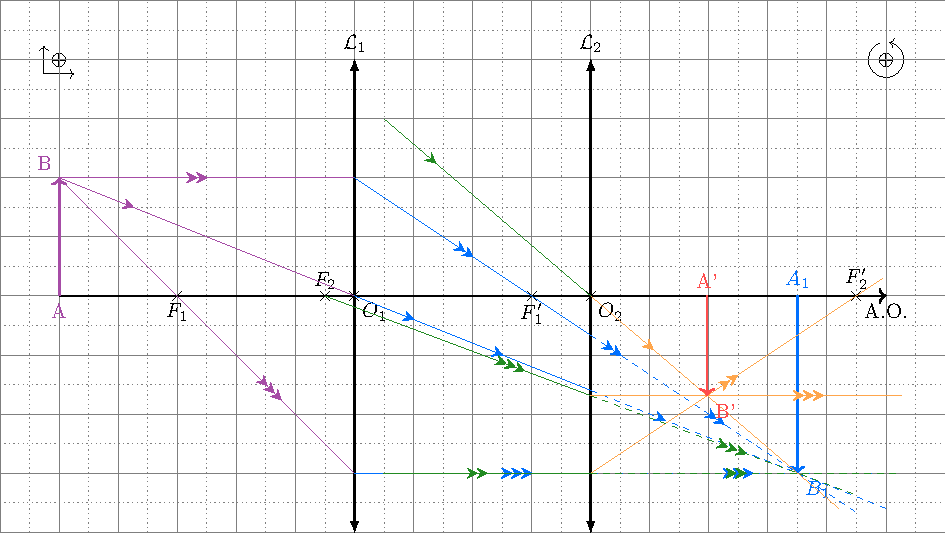
\includegraphics[width=.85\linewidth]{asso_lent-a.pdf}
        \captionof{figure}{Association de lentilles convergentes}
        \label{fig:asso_lent-conv}
    \end{center}
\end{exem}
\begin{exem}[label=exem:asso_lent]{association quelconque de lentilles
    mixées}

    On schématise l'association par $\ABb \opto{\Lc_1}{O_1} \ABa
    \opto{\Lc_2}{O_2} \ABp$. On part d'un objet réel pour avoir $\ABa$
    \textbf{image virtuelle pour $\Lc_1$} mais \textbf{objet réel pour $\Lc_2$},
    et finalement $\ABp$ image virtuelle.

    \tcblower
    \begin{center}
        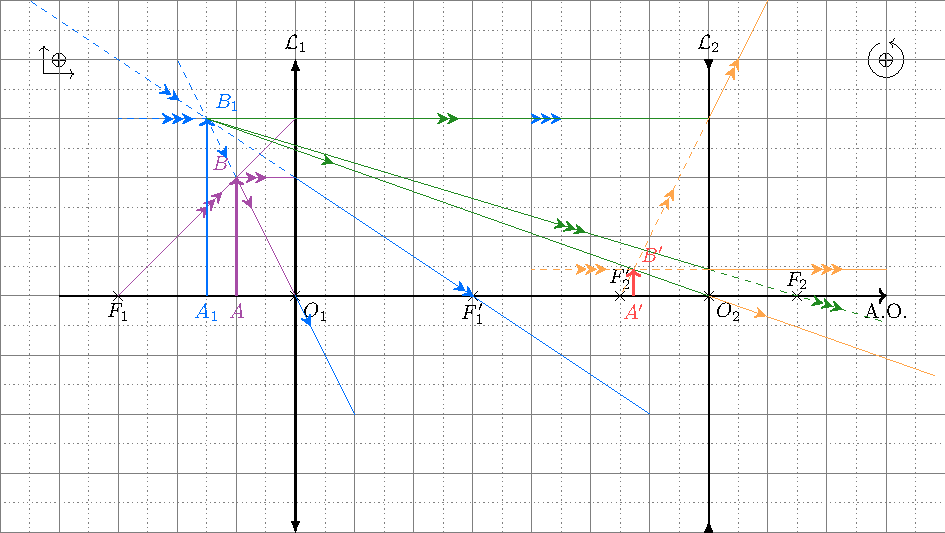
\includegraphics[width=.85\linewidth]{asso_lent-b.pdf}
        \captionof{figure}{Association de lentilles mixées}
        \label{fig:asso_lent-mix}
    \end{center}
\end{exem}

\begin{ror}[label=ror:microscope, hand]{microscope}

    Un microscope est une association de deux lentilles convergentes qui donne
    une image à l'infini d'un objet à distance finie~: $\ABb \opto{\Lc_1}{O_1}
    \ABa \opto{\Lc_2}{O_2} +\infty$
\end{ror}

\subsection{Lunettes astronomiques}
\subsubsection{Définition}

\begin{defi}[label=lunettekepler, sidebyside, righthand width=.6\linewidth]{{
            lunettes de Kepler et de Galilée, système afocal}}

    On appelle lunette astronomique un système optique composé d'une lentille
    convergente appelée \textbf{objectif} (dirigée vers l'objet) et d'une
    lentille appelée \textbf{oculaire} (dirigée vers l'œil), telle qu'un
    \textbf{objet à l'infini donne une image à l'infini}~: on appelle ce type de
    système un système \textbf{afocal}. Une lunette est dite de \textbf{Kepler}
    si l'oculaire est \textbf{convergent}, et de \textbf{Galilée} s'il est
    \textbf{divergent}.

    \tcblower
    \begin{center}
        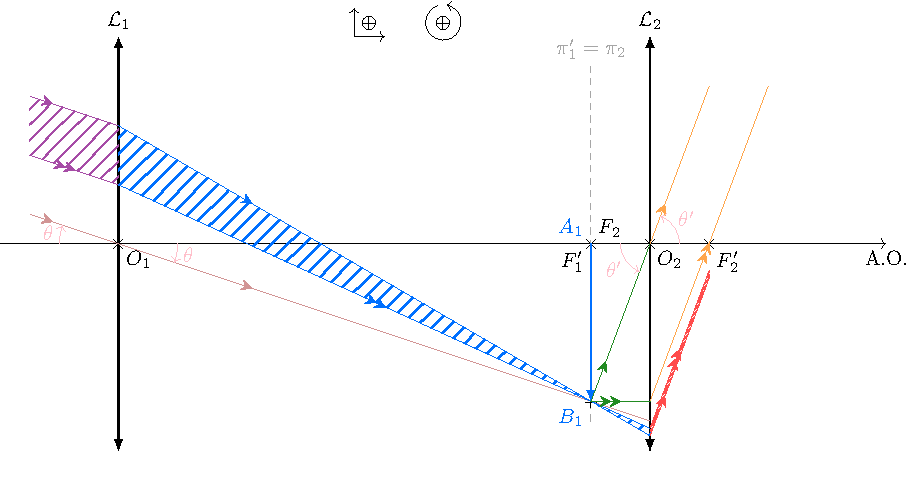
\includegraphics[width=\linewidth]{kepler}
        \captionof{figure}{Schéma d'une lunette de Kepler.}
        \label{fig:kepler}
    \end{center}
\end{defi}

\subsubsection{Caractéristiques}

\begin{tcbraster}[raster columns=4, raster equal height=rows]
    
    \begin{defi}[label=def:encombrement]{encombrement}
        On appelle \textit{encombrement} la distance $\obar{O_1O_2}$ entre
        l'objectif et l'oculaire.
    \end{defi}
    \begin{exem}[label=exem:encombrement, raster multicolumn=3]{calcul d'encombrement}

        Soit l'objectif $\Lc_1$ de centre $O_1$ et de vergence $V_1 =
        \SI{3.125}{\delta}$, et l'oculaire $\Lc_2$ de centre $O_2$ et de
        vergence $V_2 = \SI{25}{\delta}$. Quel est l'encombrement du système~?

        \tcblower
        \begin{exemside}
            Le système étant afocal, on a\\
            \begin{tikzpicture}[]
                \node[] (AB) at (0,0) {$\ABb$};
                \node[] (A_1B_1) at (2,0) {$\ABa$};
                \node[] (A'B') at (4,0) {$\ABp$};
                \draw[->] (AB) -- (A_1B_1)
                    node [midway, above] {$\Lc_1$}
                    node [midway, below] {$O_1$};
                \draw[->] (A_1B_1) -- (A'B')
                    node [midway, above] {$\Lc_2$}
                    node [midway, below] {$O_2$};
                \node[below=0.3, Purple!70] (ABb) at (AB) {$-\infty$};
                \node[below=0.3, color=brandeisblue] (A1B1b) at (A_1B_1) {$A_1 = F'_1$};
                \node[below=0.3, ForestGreen] (A1B1bb) at (A1B1b) {$A_1 = F_2$};
                \node[below=0.3, orange!70] (A'B'b) at (A'B') {$A' = +\infty$};
                \draw[->, Purple!70] (ABb) to[bend right] (A1B1b.west);
                \draw[->, orange!70] (A'B'b) to[bend left] (A1B1bb.east);
            \end{tikzpicture}
            \tcblower
            \vspace{-1cm}
            \begin{align*}
                \obar{O_1O_2} & = \obar{O_1F_1'} + \obar{F_2O_2}\\
                              & = f'_1 + f'_2\\
                              & = \frac{1}{V_1} + \frac{1}{V_2}\\
                \obar{O_1O_2} & = \SI{36}{cm}
            \end{align*}
        \end{exemside}
    \end{exem}
\end{tcbraster}
\begin{tcbraster}[raster columns=5, raster equal height=rows]
    \begin{prop}[label=prop:gross_lunette]{grossissement}
        Pour les lunettes, on a $G$ tel que
        \begin{empheq}[box=\fbox]{equation*}
            G = \frac{f'_1}{-f'_2}
        \end{empheq}
    \end{prop}
    \begin{demo}[label=demo:gross_lunette, raster multicolumn=2]{grossissement}
        À partir de la figure~\ref{fig:kepler} et en considérant des petits
        angles, on a $\theta' = \dfrac{\ABa}{\obar{O_2F_2}}$, et $\theta =
        \dfrac{\ABb}{\obar{O_1F'_1}}$~; ainsi, comme $G =
        \frac{\theta'}{\theta}$, et que $\obar{O_2F_2} = -f'_2$, on a
        directement le résultat.
    \end{demo}
    \begin{rema}[label=rema:gross_lunette, raster multicolumn=2]{grossissement}
        Comme on s'intéresse à des points à l'infini, c'est le grossissement qui
        nous intéresse. Cette équation est la même pour les deux lunettes, mais
        \textbf{$f'_2 < 0$ pour une lentille divergente}~: l'une donne donc une
        image droite et l'autre renversée.
    \end{rema}
\end{tcbraster}
\begin{tcbraster}[raster columns=2, raster equal height=rows]
    \begin{defi}{Cercle oculaire}

        On appelle \textbf{cercle oculaire} l'\textbf{image de la monture de
        l'objectif donnée par l'oculaire}.

    \end{defi}
    \begin{inte}{Utilité du cercle oculaire}
        Il correspond à la section la plus étroite du faisceau sortant de
        l'oculaire, où l'œil reçoit le maximum de lumière.  
    \end{inte}
\end{tcbraster}
\begin{exem}[label=exem:co, sidebyside]{lunette et cercle oculaire}
    \begin{center}
        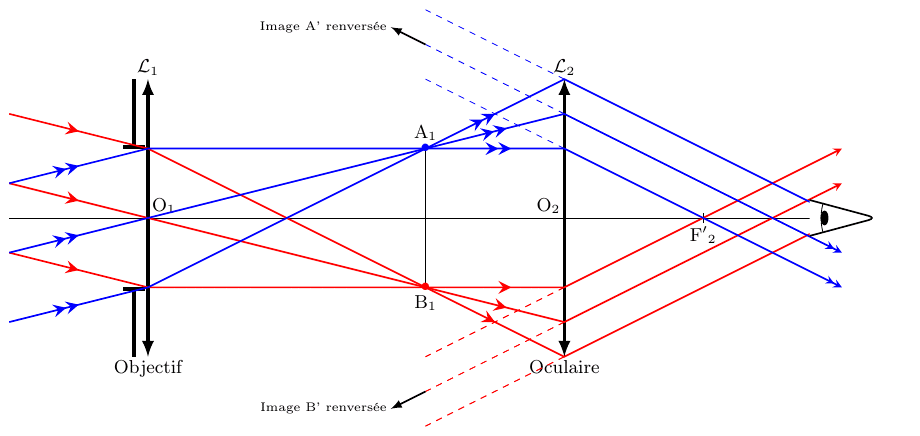
\includegraphics[width=\linewidth]{kepler_2obj}
        \captionof{figure}{Images de 2 points objets à l'infini.}
        \label{fig:kepler_2obj}
    \end{center}
    \tcblower
    \begin{center}
        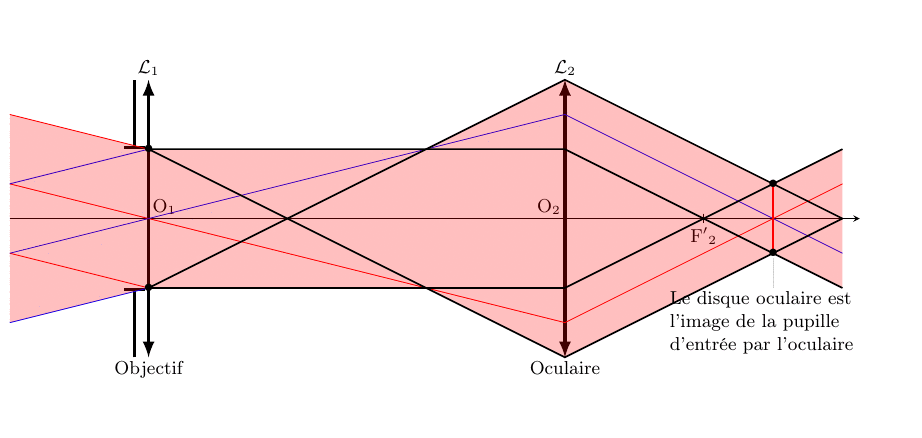
\includegraphics[width=\linewidth]{kepler_co}
        \captionof{figure}{Schématisation du cercle oculaire.}
        \label{fig:kepler_co}
    \end{center}
\end{exem}


\end{document}
